% (c) 2014 Michiel Appelman
\section{Conclusion} % (fold)
\label{sec:conclusion}

%The networking industry sees their networks growing and changing. 
This research has defined the \ac{dvpn} service as a way to adapt to this growth by providing flexibility and manageability to these networks. This is accomplished by providing operators with interfaces towards their networking equipment allowing them to get more granular control.

While discussing the implementation of \ac{mpls} for \acp{dvpn} we found that the stack has gotten more and more complex due to the accumulation of protocols providing additional features. These protocols and techniques have been designed and integrated with each other over the last years. The dependencies they have on each other have made changing or extending these protocols very difficult and thus the complexity of \acp{nms} have increased as well. This has also been caused by the lack of a common interface towards the devices, meaning that portability of these systems is low. These limitations will make implementing \acp{dvpn} in a real-life scenario a complex undertaking.

We also described how a \ac{dvpn} service can be implemented in \ac{sdn}. The design requires the development of several applications to be used by the controller to provide this service. However, by doing so the operator is provided with a more manageable interface towards its network. Or at least to an abstraction thereof, presented by the controller and its applications. 

Using these abstractions and the global network view operators can also develop their own control programs to provide new features in the network. We have shown an example implementation to provide \ac{mac} address exchange between \acp{pe}, a functionality that is still in draft for the \ac{mpls} architecture (\ac{evpn} \cite{evpn}). However, the \ac{sdn} architecture still lacks a definition for the Northbound interface which limits the portability of the applications and thus their flexibility.

The OpenFlow protocol has been described and we have used it in our design to provide the interface from the controller to the network devices. The implementation uses \ac{mpls} labels to separate traffic flows and provision paths over the network. Additionally combined with the controller and the applications it can accommodate most other features of the \ac{dvpn} service. However, the simplicity of the protocol also has a down side in the form of preventing forwarding plane monitoring. This means that in to detect failures in the network path, the controller needs to be consulted yielding higher recovery times \cite{scalable-fault}.

To summarize the benefits and limitations of using both implementations we have compiled a list containing the advantages and disadvantages of the \ac{mpls} and OpenFlow implementation. Below is the list for the \ac{mpls} protocol stack  with the advantages on the left and disadvantages on the right side:

\vspace{5 mm}

\begin{minipage}[t]{0.5\textwidth}
\begin{itemize}[label=\checkmark]
	\item Known technology which is mature, well supported and understood throughout the networking industry.
	\item Ready to be used for carrier ethernet networks, providing operators with functionalities such \ac{frr} and \ac{ecmp}.
\end{itemize}
\end{minipage}%
\begin{minipage}[t]{0.5\textwidth}
\begin{itemize}[label=$\times$]
	\item Large protocol stack with intricate dependencies.
	\item Lack of a consistent management interface towards the networking devices.
	\item Deploying an \ac{nms} to configure this stack and also be portable to different networking devices will lead to a complex piece of software, equal in inflexibility to the \ac{mpls} stack itself.
	\item The \ac{evpn} standard providing \ac{cmac} exchange and Unknown Unicast filtering is still in draft.
\end{itemize}
\end{minipage}

%\vspace{5 mm}
\clearpage
The list for implementing the \ac{dvpn} service using an \ac{sdn} architecture with OpenFlow as the Southbound interface is shown below:

\vspace{5 mm}

\begin{minipage}[t]{0.5\textwidth}
\begin{itemize}[label=\checkmark]
	\item Ability to learn from the \ac{mpls} implementation, while being able to improve upon the architecture \cite{ss} by adding operator control.
	\item Provide controller and applications with global network view, allowing for more granular control of network resources and paths.
	\item Use network abstractions to develop applications providing new features, e.g.\ \ac{mac} Exchange on \acp{pe}.
	\item Since version 1.1 OpenFlow allows rate limiting per Flow, giving more control over network resources at aggregation points.
\end{itemize}
\end{minipage}%
\begin{minipage}[t]{0.5\textwidth}
\begin{itemize}[label=$\times$]
	\item Centralization limits the independent decision-making of network devices, which harms failure recovery procedures, e.g.\ forwarding plane monitoring.
	\item The Northbound interface connecting the applications to the controller has not be defined, limiting portability.
	\item The East/westbound interface between controllers is not standardized, limiting scalability.
	\item By removing the intelligence from the networking devices, functionalities providing that intelligence have to be developed using the centralized applications.
\end{itemize}
\end{minipage}

\vspace{5 mm}

% section conclusion (end)

\subsection{Recommendations} % (fold)
\label{sub:recommendations}

Using OpenFlow and \ac{sdn} to implement \ac{dvpn} services or use it in any carrier network will require some further development on the interfaces to and from the controller. First, the OpenFlow southbound interface is still limited by a set of functionalities that lacks features that are required in the forwarding plane. However, the \ac{sdn} architecture allows for the definition of abstractions for the network. This has been shown by the OpenDaylight architecture using the Service Abstraction Layer, as can be seen in Figure~\ref{fig:opendaylight}. Using these abstractions, the available interfaces towards the networking devices may be extended by new standards or vendor specific interfaces which do provide these functions. It should be noted however that the OpenDaylight specification is in its infancy but is a step in the right direction.

\begin{figure}[!h]
	\centering
	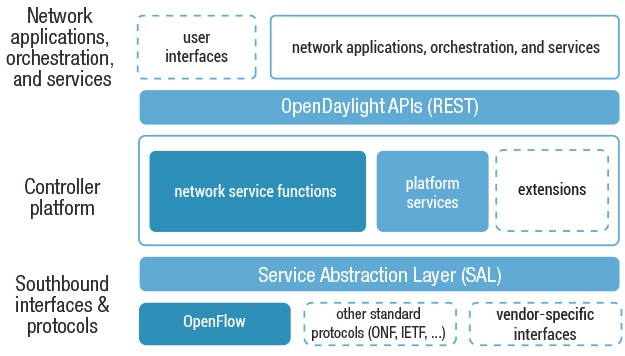
\includegraphics[width=10cm]{./includes/opendaylight.jpg}
	\caption{The proposed OpenDaylight architecture.}
	\label{fig:opendaylight}
\end{figure}

Next, the northbound interface will need to be defined. Here the OpenDaylight proposes a standardized \ac{api} to be implemented on the controller platform. By doing so, the applications that are developed for certain controller versions can be ported to other platforms. This clear separation allows for the evolution of the individual components, adding to the flexibility of the network. This also applies to the East/westbound interface. When these are standardized, vendors and developers will be able to create interoperable controllers and applications. Until that time, the improved flexibility and scalability of the \ac{sdn} is not as veritable as proponents suggest.

Implementing \acp{dvpn} using OpenFlow also leads to other questions which need to be answered for specific implementations of controllers, hardware and applications. 
This research has taken a theoretical approach to implementing new carrier services without focussing on specific hardware and software implementations. Scalability and efficiency of different applications and hardware implementations will need to be researched when looking to implement \acp{dvpn} using \ac{sdn}. 

% subsection recommendations (end)

\subsection{Future Work} % (fold)
\label{sub:future_work}

Apart from the research that has to be done on implementation-specific level, more  research can be done on how \ac{sdn} and OpenFlow can be used to implement multi-domain \acp{vpn}. A multi-domain \ac{vpn} service provides \acp{vpn} to customers of different \acp{sp}, requiring them to exchange information on these customers. This information exchange will need to happen with a certain trust level and using \acp{api} that provide \acp{sp} with their required security. Implementing such a service using the \ac{mpls} architecture will be less straightforward and desirable than the \ac{sdn} architecture, as the \ac{mpls} architecture will need to provide deep access to the sensitive forwarding plane of the network. However, the feasibility and implications of implementing such a service using \ac{sdn} may also require more research.

Another feature that might be looked into further is the statistics of the OpenFlow flows in the network when trying to implement realtime metering. This feature can be used to get more timely statistics of traffic flowing over the network and acting upon those values. For instance, a certain \ac{vpn} may have a data limit imposed by the operator on the amount of traffic exchanged over the network in a certain time frame. By using realtime monitoring, the operator can act upon exceeding the threshold by stopping the traffic without have to wait for statistics gathering scripts. 

Finally, there are still other carrier network obstacles that \ac{sdn} promises to solve. One of which is mobility of customer devices. Research into how OpenFlow might provide this functionality efficiently would also be of distinct value to the industry.

% subsection future_work (end)